\question{طراحی سامانه‌ی رقمی تشخیص عدد آینه‌ای}

\begin{enumerate}
    \item \textbf{نمودار \lr{ASM} طراحی شده به این صورت می‌باشد:}
          \begin{figure}[H]
              \centering
              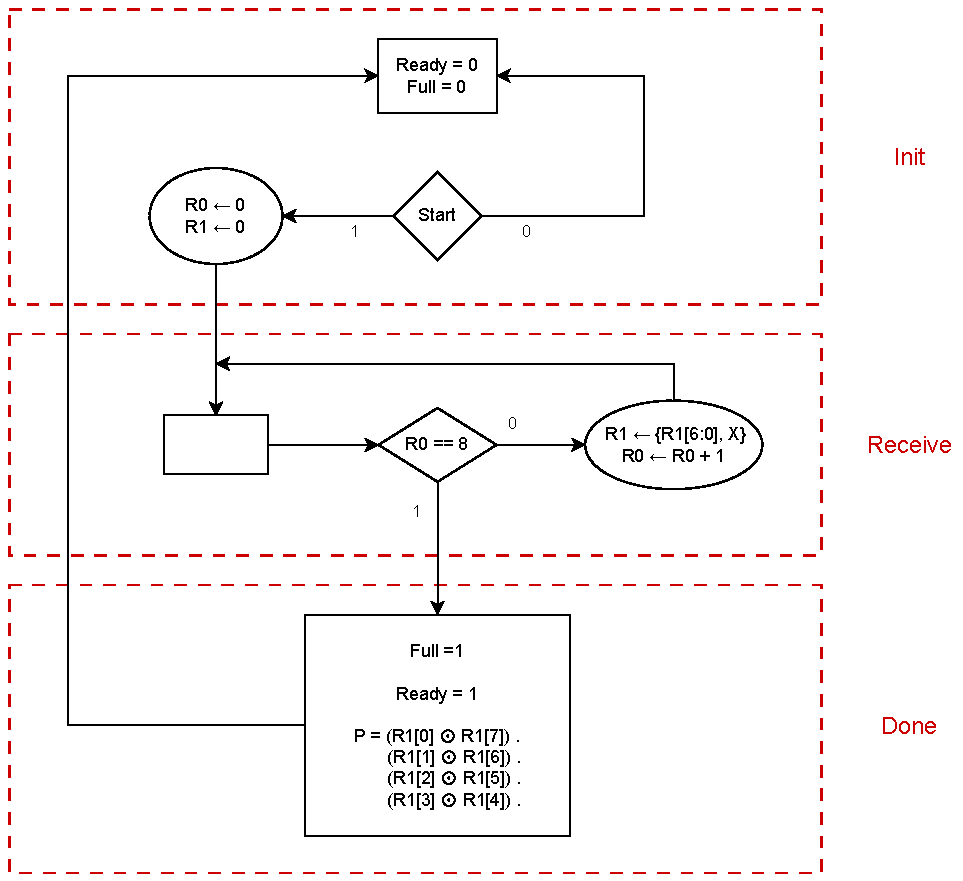
\includegraphics[width=0.7\textwidth]{assets/Q1-ASM.pdf}
              \caption{\lr{ASM Chart}ِ سامانه تشخیص عدد آینه‌ای}
          \end{figure}
          این طراحی، شامل 3 \lr{ASM Block} می‌باشد:
          \begin{itemize}
              \item \textbf{\lr{Init}:} حالت اولیه‌ی سیستم است. در این حالت سیگنال‌های \lr{Ready} و \lr{Full} در وضعیت صفر قرار دارند و منتظر می‌مانیم تا سیگنال \lr{Start} فعال شود. به محض فعال شدن \lr{Start}، رجیستر‌های \lr{R0} و \lr{R1} را ریست کرده (مقدار آن‌ها را صفر می‌کنیم) تا فرآیند دریافت داده آغاز شود. در اینجا \lr{R0} به عنوان شمارنده‌ی تعداد بیت‌های دریافتی و \lr{R1} به عنوان ثباتی که الگوی ورودی را نگه می‌دارد، عمل می‌کنند.
              \item \textbf{\lr{Receive}:} در این بخش، در هر چرخه‌ی ساعت، مقدار فعلی سیگنال \lr{X} را دریافت کرده، محتوای \lr{R1} را یک واحد به سمت چپ شیفت می‌دهیم و مقدار \lr{X} را در کم‌ارزش‌ترین بیت (\lr{LSB}) قرار می‌دهیم. همزمان، مقدار شمارنده \lr{R0} را یک واحد افزایش داده و بررسی می‌کنیم که آیا مقدار آن به 8 رسیده است یا خیر (شرط $\text{\lr{R0}} == 8$). اگر 8 بیت کامل دریافت نشده باشد، در همین حالت می‌مانیم و اگر دریافت کامل شده باشد، وارد بلاک بعدی می‌شویم.
              \item \textbf{\lr{Done}:} در این مرحله، فرآیند دریافت پایان یافته است؛ لذا سیگنال‌های \lr{Full} و \lr{Ready} یک می‌شوند. سیگنال \lr{P} نیز توسط یک مدار ترکیبی از روی بیت‌های \lr{R1} ارزیابی می‌شود تا مشخص شود آیا داده‌ی دریافتی آینه‌ای است یا خیر. در نهایت، سیستم در چرخه‌ی بعدی به حالت \lr{Init} بازمی‌گردد.
          \end{itemize}

    \item \textbf{سنتز بخش مسیر داده (\lr{Data Path}):}
          \begin{figure}[H]
              \centering
              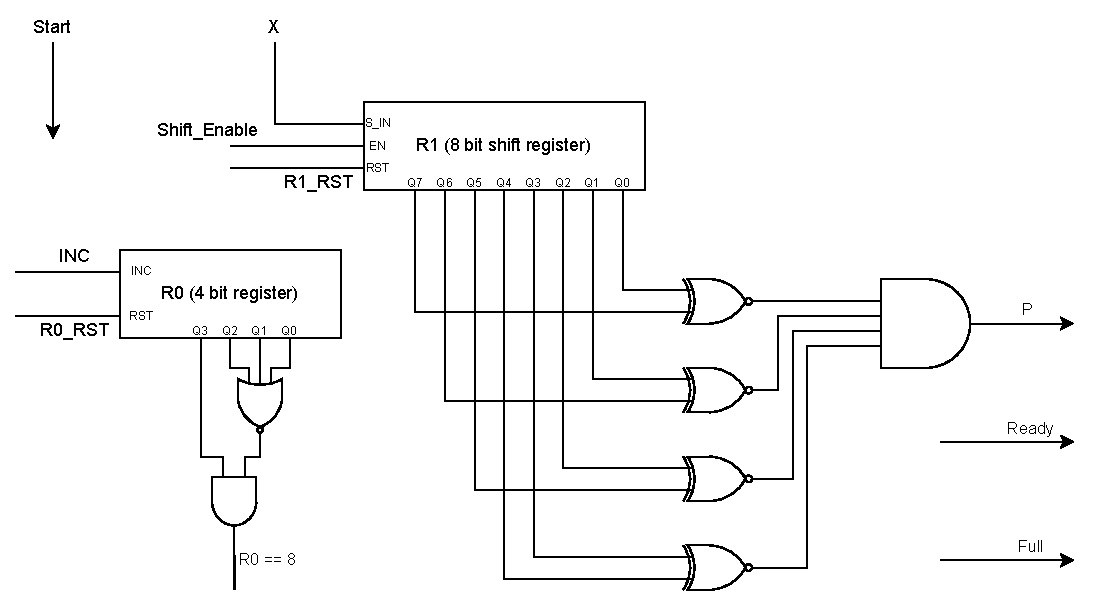
\includegraphics[width=1.0\textwidth]{assets/Q1-synthes-DP.pdf}
              \caption{بخش مسیر داده (\lr{Data Path})}
          \end{figure}
          \begin{itemize}
              \item ثبات \lr{R1} باید یک الگوی 8 بیتی را ذخیره کرده و قابلیت شیفت به چپ داشته باشد. بنابراین از یک \lr{Shift Register} هشت بیتی با قابلیت \lr{Serial In} استفاده می‌کنیم. سیگنال \lr{X} به ورودی این ثبات متصل می‌شود. پایه‌های \lr{RST} (برای صفر کردن اولیه) و \lr{EN} (برای فعال‌سازی شیفت) در مدار تعبیه شده‌اند که توسط واحد کنترل مدیریت می‌شوند.
              \item سیگنال \lr{P} نمایانگر آینه‌ای بودن محتوای \lr{R1} است. یک عدد 8 بیتی زمانی آینه‌ای است که بیت‌های متقارن آن (بیت 0 با 7، بیت 1 با 6 و غیره) با هم برابر باشند. بنابراین با 4 گیت \lr{XNOR} (برای بررسی برابری هر جفت) و یک گیت \lr{AND} به راحتی می‌توانیم سیگنال \lr{P} را تولید کنیم:
                    \begin{align*}
                        P = & (\text{\lr{R1}}[0] \odot \text{\lr{R1}}[7]) \cdot \\
                            & (\text{\lr{R1}}[1] \odot \text{\lr{R1}}[6]) \cdot \\
                            & (\text{\lr{R1}}[2] \odot \text{\lr{R1}}[5]) \cdot \\
                            & (\text{\lr{R1}}[3] \odot \text{\lr{R1}}[4])
                    \end{align*}
              \item شمارنده \lr{R0} وظیفه دارد تعداد بیت‌های دریافتی را از 0 تا 8 بشمارد. بنابراین یک ثبات 4 بیتی برای این منظور کفایت می‌کند. این ثبات دارای پایه‌های \lr{INC} (برای افزایش مقدار) و \lr{RST} (برای صفر شدن) است. برای تشخیص شرط اتمام دریافت ($\text{\lr{R0}} == 8$)، باید زمانی که بیت‌های کم‌ارزش صفر و باارزش‌ترین بیت یک است را تشخیص دهیم. این سیگنال با منطق ترکیبی زیر ساخته می‌شود:
                    \begin{align*}
                        (R0 == 8) = \text{\lr{R0}}[3] \cdot \overline{(\text{\lr{R0}}[2] + \text{\lr{R0}}[1] + \text{\lr{R0}}[0])}
                    \end{align*}
          \end{itemize}

          \textbf{سنتز واحد کنترل (\lr{Control Unit}):}
          \begin{figure}[H]
              \centering
              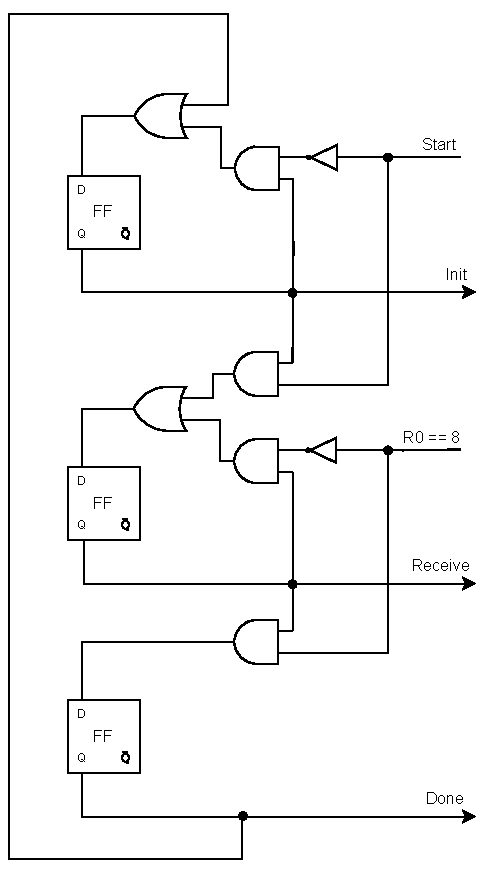
\includegraphics[width=0.5\textwidth]{assets/Q1-synthes-CU.pdf}
              \caption{واحد کنترل (\lr{Control Unit})}
          \end{figure}
          سیستم ما شامل سه \lr{ASM Block} است. برای پیاده‌سازی واحد کنترل با رویکرد \lr{One-Hot}، به 3 فلیپ‌فلاپ از نوع \lr{D} نیاز داریم که هر کدام نماینده‌ی یکی از حالت‌ها هستند. در این روش، در هر لحظه یک و تنها یک فلیپ‌فلاپ مقدار 1 دارد:
          \begin{itemize}
              \item \textbf{حالت \lr{Init}:} سیستم زمانی در این حالت می‌ماند که در همین حالت باشد و \lr{Start} صفر باشد، و یا اینکه سیستم از حالت \lr{Done} به این حالت بازگردد.
                    \begin{align*}
                        \text{\lr{Init}}^{+} = (\text{\lr{Init}} \cdot \overline{\text{\lr{Start}}}) + \text{\lr{Done}}
                    \end{align*}

              \item \textbf{حالت \lr{Receive}:} سیستم زمانی وارد این حالت می‌شود که در حالت \lr{Init} باشیم و \lr{Start} فعال شود. همچنین تا زمانی که شمارنده به 8 نرسیده باشد ($\text{\lr{R0}} \neq 8$)، در همین حالت باقی می‌مانیم.
                    \begin{align*}
                        \text{\lr{Receive}}^{+} = (\text{\lr{Init}} \cdot \text{\lr{Start}}) + (\text{\lr{Receive}} \cdot \overline{(\text{\lr{R0}} == 8)})
                    \end{align*}

              \item \textbf{حالت \lr{Done}:} سیستم تنها زمانی وارد این حالت می‌شود که در حالت \lr{Receive} باشیم و شرط دریافت 8 بیت ($\text{\lr{R0}} == 8$) برقرار شود.
                    \begin{align*}
                        \text{\lr{Done}}^{+} = \text{\lr{Receive}} \cdot (\text{\lr{R0}} == 8)
                    \end{align*}
          \end{itemize}

          \textbf{سیگنال‌های فرمان مسیر داده (\lr{Command Signals}):}
          واحد کنترل از طریق تولید سیگنال‌های فرمان، عملکرد اجزای مسیر داده را در هر حالت مدیریت می‌کند. با توجه به نمودار \lr{ASM} و منطق استخراج‌شده، این سیگنال‌ها به کمک گیت‌های منطقی ترکیبی از روی حالات فلیپ‌فلاپ‌ها به شرح زیر تولید می‌شوند:
          \begin{itemize}
              \item \textbf{سیگنال‌های ریست (\lr{R1\_RST} و \lr{R0\_RST}):} این دو سیگنال وظیفه دارند ثبات حافظه و شمارنده را در ابتدای کار صفر کنند. این عمل تنها زمانی رخ می‌دهد که سیستم در حالت \lr{Init} قرار داشته باشد و سیگنال شروع (\lr{Start}) فعال گردد:
                    \begin{align*}
                        \text{\lr{R1\_RST}} = \text{\lr{R0\_RST}} = \text{\lr{Init}} \cdot \text{\lr{Start}}
                    \end{align*}
              \item \textbf{سیگنال‌های فعال‌ساز فرآیند (\lr{Shift\_Enable} و \lr{INC}):} برای شیفت دادن داده‌ی ورودی به درون ثبات \lr{R1} و همزمان افزایش شمارنده‌ی \lr{R0}، باید سیستم در حالت \lr{Receive} بوده و هنوز دریافت ۸ بیت کامل نشده باشد ($\text{\lr{R0}} \neq 8$):
                    \begin{align*}
                        \text{\lr{Shift\_Enable}} = \text{\lr{INC}} = \text{\lr{Receive}} \cdot \overline{(\text{\lr{R0 == 8}})}
                    \end{align*}
              \item \textbf{سیگنال‌های اعلام وضعیت (\lr{Ready} و \lr{Full}):} این دو سیگنال خروجی‌های نهایی سیستم هستند که نشان‌دهنده‌ی پایان موفقیت‌آمیز فرآیند دریافت و معتبر بودن خروجی \lr{P} می‌باشند. بنابراین به محض ورود به حالت \lr{Done} فعال می‌شوند:
                    \begin{align*}
                        \text{\lr{Ready}} = \text{\lr{Full}} = \text{\lr{Done}}
                    \end{align*}
          \end{itemize}

          \textbf{مدار کامل سامانه (اتصال واحد کنترل و مسیر داده):}
          با ترکیب و اتصال بخش‌های سنتز شده‌ی مسیر داده (\lr{Data Path}) و واحد کنترل (\lr{Control Unit}) از طریق سیگنال‌های فرمان فوق، شماتیک نهایی و کامل مدار به صورت زیر حاصل می‌شود:
          \begin{figure}[H]
              \centering
              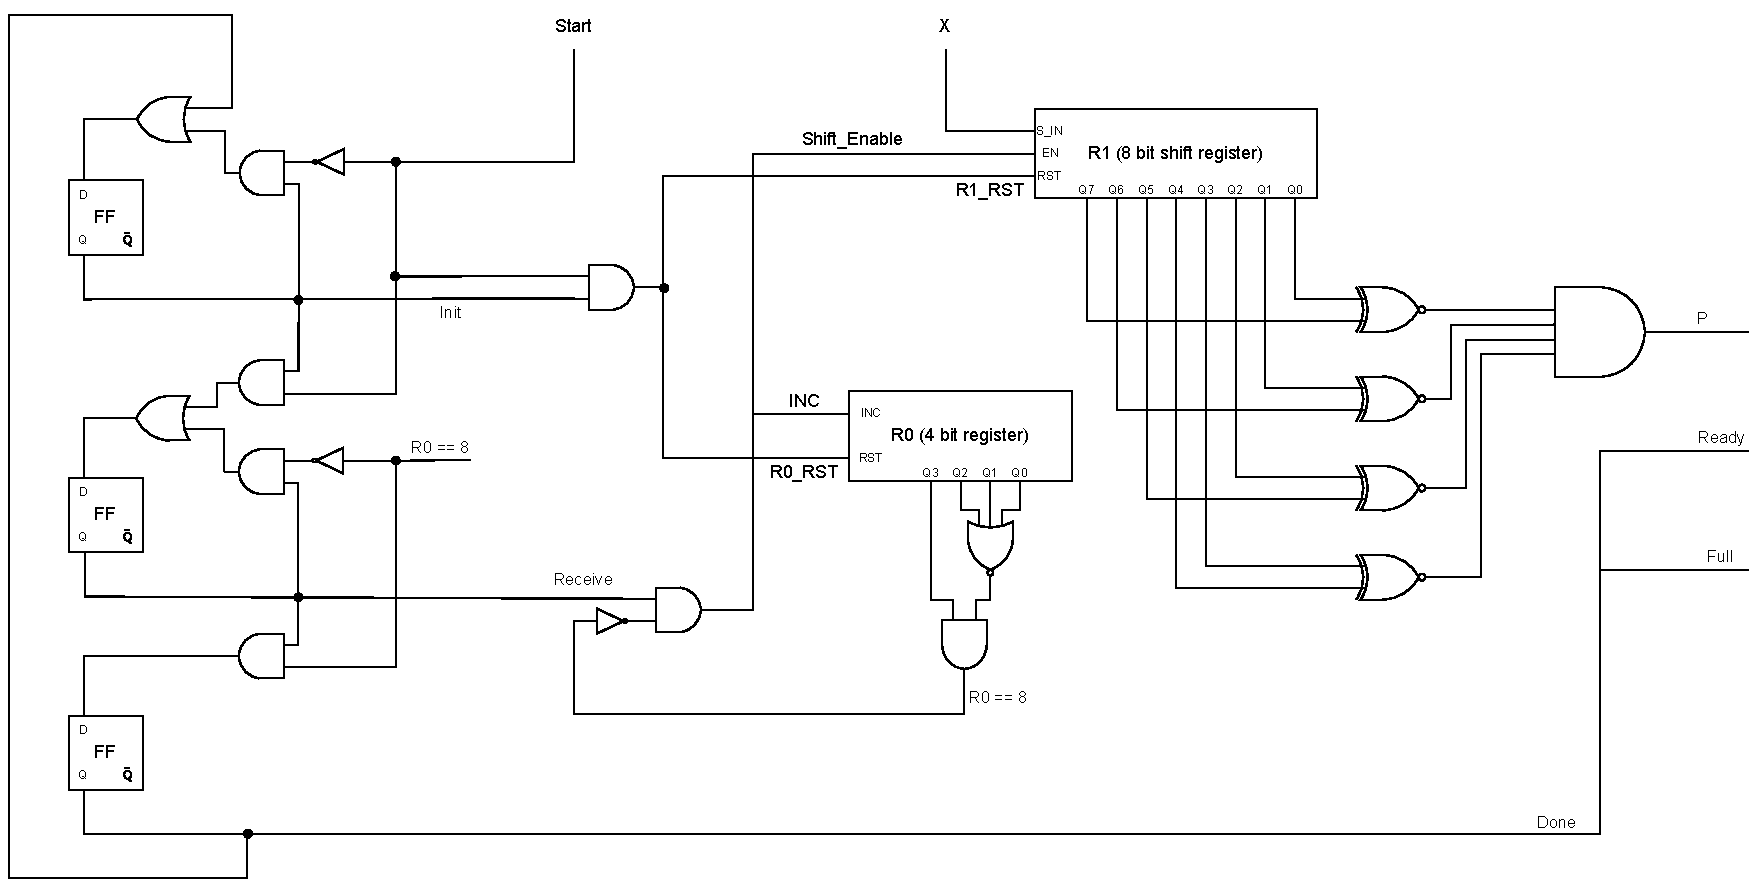
\includegraphics[width=1.0\textwidth]{assets/Q1-circuit.pdf}
              \caption{شماتیک کامل مدار سامانه تشخیص عدد آینه‌ای (شامل \lr{CU} و \lr{DP})}
          \end{figure}

          \pagebreak

    \item \textbf{نمودار و جدول انتقال حالت:}
          \begin{figure}[H]
              \centering
              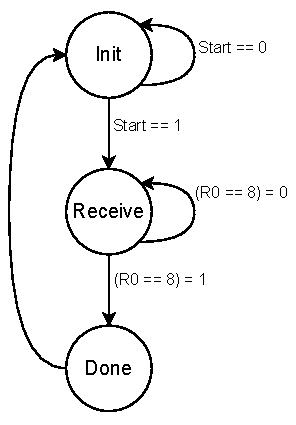
\includegraphics[width=0.35\textwidth]{assets/Q1-SM.pdf}
              \caption{نمودار انتقال حالت دستگاه}
          \end{figure}
          بر اساس نمودار \lr{ASM} و طراحی واحد کنترل، جدول انتقال حالت و خروجی‌های سیستم به شکل زیر استخراج می‌شود. خروجی‌های کنترلی مسیر داده (\lr{Control Signals}) به طور مستقیم به حالت‌های فعلی و شرایط گذار وابسته هستند:
          \begin{table}[H]
              \centering
              \resizebox{\textwidth}{!}{%
                  \begin{tabular}{|c|c|c|c||c|c|c||c|}
                      \hline
                      \multicolumn{4}{|c||}{\textbf{خروجی‌ها و \lr{command} ها}} &
                      \multicolumn{1}{c|}{\textbf{حالت بعدی}}                   &
                      \multicolumn{2}{c||}{\textbf{ورودی‌ها}}                    &
                      \multicolumn{1}{c|}{\textbf{حالت فعلی}}                                                                     \\
                      \hline
                      \textbf{\lr{P}}                                           &
                      \textbf{\lr{Ready}, \lr{Full}}                            &
                      \textbf{\lr{Shift\_EN}, \lr{INC}}                         &
                      \textbf{\lr{R1\_RST}, \lr{R0\_RST}}                       &
                      \textbf{\lr{Next State}}                                  &
                      \textbf{$(R0==8)$}                                        &
                      \textbf{\lr{Start}}                                       &
                      \textbf{\lr{State}}                                                                                         \\
                      \hline
                      X                                                         & 0 & 0 & 0 & \lr{Init}    & X & 0 & \lr{Init}    \\
                      X                                                         & 0 & 0 & 1 & \lr{Receive} & X & 1 & \lr{Init}    \\
                      X                                                         & 0 & 1 & 0 & \lr{Receive} & 0 & X & \lr{Receive} \\
                      X                                                         & 0 & 0 & 0 & \lr{Done}    & 1 & X & \lr{Receive} \\
                      \text{محاسبه در مدار ترکیبی}                              & 1 & 0 & 0 & \lr{Init}    & X & X & \lr{Done}    \\
                      \hline
                  \end{tabular}%
              }
              \caption{جدول انتقال حالت و خروجی‌های واحد کنترل}
          \end{table}

    \item \textbf{محاسبه مجموع تعداد فلیپ‌فلاپ‌های مورد نیاز:}
          برای پیاده‌سازی کل سامانه به فلیپ‌فلاپ‌های زیر نیاز داریم:
          \begin{itemize}
              \item \textbf{مسیر داده (\lr{Data Path}):} ثبات \lr{R1} یک شیفت‌رجیستر 8 بیتی است که نیاز به 8 فلیپ‌فلاپ دارد. شمارنده \lr{R0} نیز برای شمارش از 0 تا 8 به 4 فلیپ‌فلاپ نیاز دارد. (مجموعاً 12 عدد)
              \item \textbf{واحد کنترل (\lr{Control Unit}):} از آنجایی که از روش \lr{One-Hot} برای 3 حالت (\lr{Init}, \lr{Receive}, \lr{Done}) استفاده کرده‌ایم، به 3 فلیپ‌فلاپ نیاز است.
              \item \textbf{مجموع کل:} $12 + 3 = 15$ فلیپ‌فلاپ برای پیاده‌سازی کامل مدار مورد نیاز است.
          \end{itemize}
          توجه داریم که این طراحی لزوماً بهینه نبوده و با کارهایی از جمله استفاده از روش \lr{Binary Encoding} به جای \lr{One Hot} در واحد کنترل و بهینه‌تر کردن مسیر داده، می‌توان تعداد فلیپ‌فلاپ‌های استفاده شده را کاهش داد.
\end{enumerate}